\documentclass[12pt, letterpaper]{article}
\usepackage{fullpage}
\usepackage[utf8]{inputenc}
\usepackage[english]{babel}
\usepackage[usenames, dvipsnames]{color}
\usepackage{listings}
\usepackage{color}
\usepackage{hyperref}
\usepackage[toc,page]{appendix}
\usepackage{underscore}
\usepackage{csquotes}
\usepackage{graphicx}

\graphicspath{ {./images/} }
\DeclareGraphicsExtensions{.png,.pdf}

\hypersetup{
    colorlinks=true,
    linkcolor=blue,
    filecolor=magenta,
    urlcolor=cyan,
}

\urlstyle{same}

\definecolor{backcolor}{rgb}{0.95,0.95,0.95}

\lstdefinestyle{codestyle}{
    backgroundcolor=\color{backcolor},
    basicstyle=\ttfamily\normalsize,
    breaklines=false
}

\lstset{style=codestyle}

\sloppy
\hbadness=99999

\usepackage[
backend=biber,
style=alphabetic,
sorting=ynt
]{biblatex}
\addbibresource{capstone.bib}

\title{Capstone Project Proposal\\[8pt]
\normalsize{Udacity Machine Learning Nanodegree}}
\date{June 5, 2018}
\author{James Dellinger}
\begin{document}
\maketitle

\section{Domain Background}
For my capstone project I will participate in the \href{https://www.kaggle.com/c/home-credit-default-risk}{Home Credit Default Risk competition} on Kaggle\cite{kagglehomecreditcompetitionoverview}. The goal of the competition is to be able to predict the likelihood that an applicant will experience difficulty in repaying their loan. The competition is sponsored by \href{http://www.homecredit.net}{Home Credit}\cite{homecreditwebsite}, whose mission is to provide a positive and safe borrowing experience to groups of people that traditional, mainstream banks and financial institutions typically refuse to serve.

Home Credit targets a demographic that typically has no recourse but to deal with shady characters such as loan sharks when borrowing money. Many of these unbanked individuals are hard-working, well-intentioned folks who, either due to circumstances beyond their control or past mistakes, have fallen through the financial system’s cracks.

I want to live in a world where a second chance is available to anyone who would make a good faith effort to make the most of it. This is why Home Credit’s goal of providing a safe lending alternative to otherwise financially down-and-out folks resonates with me. I want to help Home Credit have the ability to expand its services to as many deserving applicants as possible.

\section{Problem Statement}
\label{problemstatement}
Home Credit needs an algorithm that will take as inputs various personal and alternative financial information originally taken from a loan applicant's profile, and then determine a probability of the applicant having at least one late payment when repaying their loan. This probability will be in the range [0.0, 1.0], where 1.0 represents a 100\% certainty that the applicant will have at least one delinquent repayment and 0.0 indicates that there is zero chance that the applicant will ever be delinquent. The algorithm will be tested on a set of 48,744 individuals who previously borrowed from Home Credit. A CSV file must be produced that contains one header row, and 48,744 prediction rows, where each prediction row contains both a user ID, the \colorbox{backcolor}{\textcolor{red}{\texttt{SKI_ID_CURR}}} column, and the probability, the \colorbox{backcolor}{\textcolor{red}{\texttt{TARGET}}} column, of that user being delinquent. The file must be formatted as follows:

\begin{lstlisting}
SK_ID_CURR,TARGET
100001,0.1
100005,0.9
100013,0.2
etc.
\end{lstlisting}

Home Credit knows which borrowers ultimately paid off their loans, and which ones had one or more late payments. A good algorithm will need to predict a high probability of delinquency for the majority of borrowers who did actually make one or more late payments. This algorithm will also need to predict a low probability of delinquency for the majority of borrowers who eventually did successfully repay their loans with no late payments.

\section{Datasets and Inputs}
This competition's dataset was provided by Home Credit Group's data scientists. It contains a wide variety of personal and financial information belonging to 356,255 individuals who had previously been recipients of loans from Home Credit. These individuals are divided into training and testing sets. The training group contains 307,511 individuals' records. The test group contains 48,744 records. The dataset is anonymized, with each individual represented by their loan ID. Any personally indentifying infomation, such as name, phone number, or address, has been omitted.

Because Home Credit targets the unbanked population, it is unable to rely on traditional measures, such as a credit score, that mainstream financial institutions use when making lending decisions. Home Credit works around this obstacle by looking at an extensive and diverse array of personal and financial information for each of its applicants. These features range from common characteristics, such as marital status, age, type of housing, region of residence, job type, and education level, to some incredibly niche characteristics, such as how many elevators are in an applicant's apartment building. Home Credit also looks at nitty gritty aspects of applicants' financial backgrounds, including month-by-month payment performance on any loans or credit card balances that the applicant has previously had with Home Credit, as well as the amount and monthly repayment balances of any loans that the applicant may have received from other lenders.

All of these features are spread across seven data tables. The main data table (application_\{train \textbar~test\}.csv) contains 120 features that comprise applicants' personal background information. The other six data tables contain applicants' previous loan and credit card balance payment histories. Detailed descriptions of each data table can be found in Appendix \ref{appendix:datatabledescriptions}. Explanations of all features in each data table are in Appendix \ref{appendix:datatablefeatures}. The following diagram provides a brief summary:

\begin{figure}[ht]
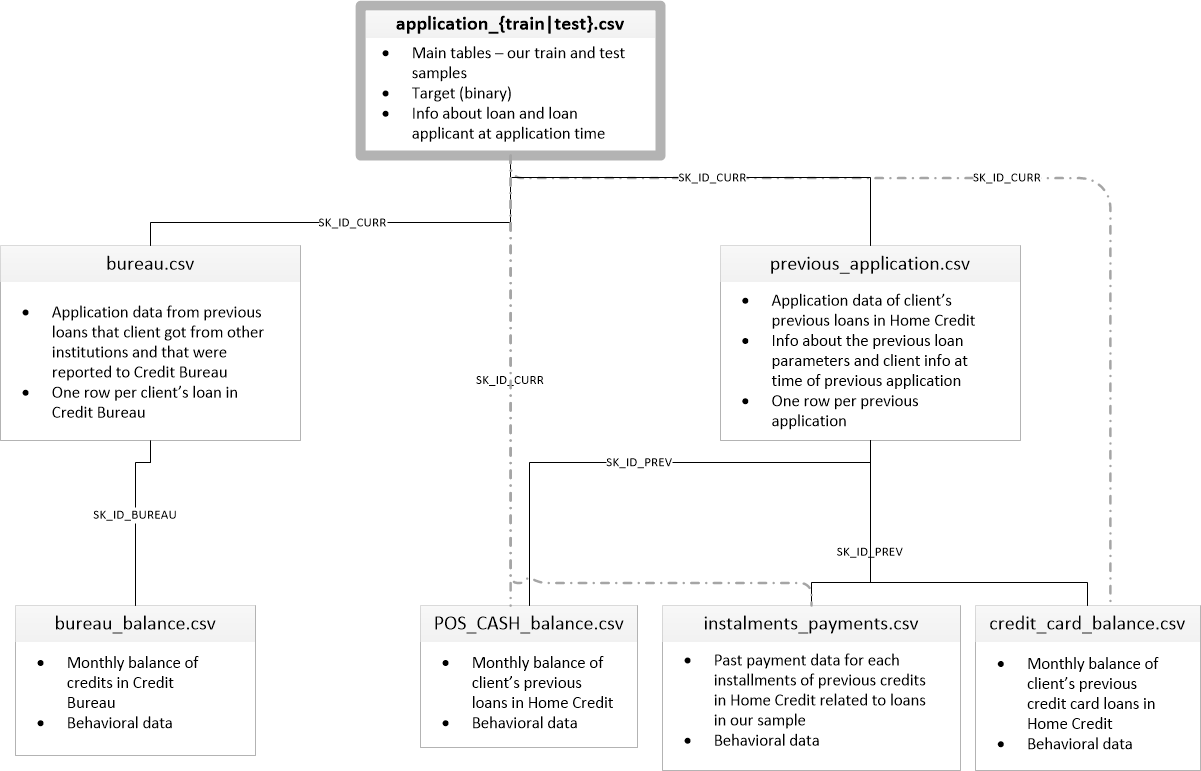
\includegraphics[width=0.9\textwidth]{homecredit}
\centering
\caption{Home Credit Data Table Relationships\cite{kagglehomecreditcompetitiondata}}
\end{figure}

\section{Solution Statement}
The solution to this competition will be an algorithm that computes delinquency probabilities (in the range [0.0,1.0]) for each of the 48,744 Home Credit borrowers in the dataset's test segment. These predictions will be stored in a CSV file that adheres to the format described in the Problem Statement above in Section \ref{problemstatement}. This algorithm will take as inputs features from the seven data tables outlined above. It will be trained on the 307,511 Home Credit borrower records that comprise the training segment. The winning algorithm will predict the highest probabilities of delinquency for the borrowers who had at least one late payment, and will predict the lowest probabilities of delinquency for the borrowers who ultimately repaid their loans with no late payments. More formally, a winning algorithm will have the highest true positive rate, or sensitivity, (correctly guessing who will be delinuent), while at the same time having a minimum false positive rate (as seldom as possible making an incorrect guess that an individual will have difficulty paying back their loan).

\section{Benchmark Model}
Solutions to this competition will be ranked on Kaggle by the area under the ROC curve between their predicted proabilities and the observed targets (whether or not the borrower was actually delinquent). An ideal benchmark would be the area under ROC curve of the prediction model employed by Home Credit's data scientists prior to this competition's debut on Kaggle. However, since Home Credit possibly considers the specifics of this model and its ROC curve area to be proprietary information, it is understandable that they were not disclosed. As a next best alternative, I will use as a benchmark the average ROC curve area of all entries on the competition's public leaderboard\cite{kagglehomecreditcompetitionpublicleaderboard} as of June 2, 2018. As of this date, there were 5,398 total entries from 1,515 participants. The average area under the ROC curves of all entries was \colorbox{backcolor}{\textcolor{red}{\texttt{0.7379}}}. I hope to design an algorithm that will meet or exceed this score.

\section{Evaluation Metric}
The area under the ROC (receiver operating characteristic) curve\cite{wikipediaroc} will be the evaluation metric for my solution to this competition. This area can range from a minimum value of 0, or 0\%, to a maximum of 1, or 100\%. The size of the area under an ROC curve indicates how good a job a classifier does of identifying a certain target segment in a dataset. An area of 1 indicates that the classifier is perfect -- that it can find every true positive (exhibiting perfect sensitivity, or recall) without making any mistakes (not accidentally labelling some true negatives as false positives), thus also giving it perfect specificity, which leads to a false positive rate (1 - specificity), of zero. An area of 0 indicates that the classifier isn't able to find and properly label any of the true positives. An area of 0.5 is the level of performance we'd expect from a classifier that randomly labels each point in the dataset -- on the whole, this classifier would make just as many mistakes (false positives) as it makes correct predictions (true positives).

\begin{figure}[ht]
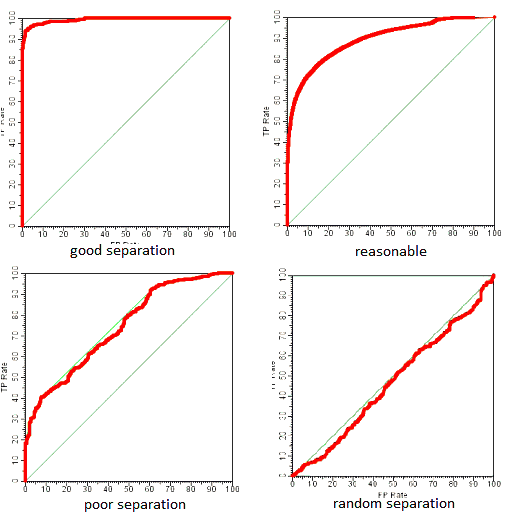
\includegraphics[width=0.5\textwidth]{roccurves}
\centering
\caption{ROC Curve Examples\cite{mlwikirocanalysis}}
\end{figure}

Because the goal of this competition is to create an algorithm that correctly identifies applicants who were delinquent in repaying their loans, area under the ROC curve is a perfectly appropriate measure of my algorithm's performance. While my target benchmark is the score of \colorbox{backcolor}{\textcolor{red}{\texttt{0.7379}}} that I mentioned above, at a bare minimum, my classifier must achieve a score of better than 0.5 -- anything less would mean that my classifier performs only as good as, or worse than, a random classifier.

\section{Project Design}
Although Home Credit provides seven data tables for this competition, for the purposes of this project I will focus most of my attention on the main data table. However, at a minimum, I will engineer at least one feature from the remaining six data tables. I may dive deeper into these other six data tables if time permits. I will structure my approach to creating a high-performing classification algorithm according to the steps in the following provisional workflow:

\renewcommand{\labelenumi}{\Roman{enumi}}
\begin{enumerate}
  \item \textbf{Data Exploration}
    \begin{enumerate}
      \item Compile lists and short descriptions of each feature in all seven of the competition's data tables.
      \item Display number of entries (rows) in each data table.
      \item Display number of features in each data table.
      \item Generate and display 5-row samples of each data table.
      \item Generate and display statistical descriptions of the numerical features of each data table that will be used by my algorithm.
      \item Investigate whether any features in any of the data tables have "NaN" entries that will need to be handled, and whether some features have sparse enough data such that the entire feature should be removed.
      \item Also investigate whether any borrowers (rows) in the main data table have 'NaN' for the majority of their feature entries. Some of these datapoints may also need to be removed.
      \item Review the statistical descriptions of each numerical feature, and ensure that there are no other unexpected numerical entries in these features, eg. a feature having some negative numbers among its entries, where only positive numbers would be expected based on how the feature was defined by Home Credit.
      \item List the numerical features in the main data table that are not already identified as being normally distributed (they may eventually need to be log-normalized).
      \item List the categorical features in the main data table that will need to be one-hot encoded.
      \item List the categorical features in the data table that are already one-hot encoded.
      \item Define at least one feature that could be engineered from the data contained in the other six data tables outside of the main data table.
    \end{enumerate}
  \item \textbf{Exploratory Visualization}
    \begin{enumerate}
      \item Plot histograms of the numerical features in the main data table, in order to confirm which ones are indeed already normally distributed.
      \item Plot histograms of the numerical features in the main data table that are supposedly not already normally distributed.
      \item Identify any outliers that will need to be addressed.
    \end{enumerate}
  \item \textbf{Algorithms and Techniques to Consider}
    \begin{enumerate}
      \item \textbf{Dimensionality Reduction}:
        \begin{enumerate}
          \item Feature transformation and dimensionality reduction using Principle Component Analysis (PCA)
          \item Dimensionality reduction using Sparse Random Projection (in case using PCA is too taxing on my compute resources)
        \end{enumerate}
        Note: Many of the features may well be correlated with each other, and thus not independent, so I cannot use a dimensionality reduction algorithm that assumes feature independence, such as Independent Component Analysis (ICA).
      \item \textbf{Learning Algorithms}:

      Any algorithm that I use will need to not only be able to simply segment the data points into the ``delinquent repayers" and ``on-time repayers" categories, but must also be able to compute the probability that each data point in the test set belongs to the ``delinquent repayers" segment. These probabilities will naturally be higher for points that the algorithm labels as ``delinquent repayers," and will be lower for the points that are labeled as ``on-time repayers." This requirement automatically eliminates algorithms such as SVM, K-Means, Hierarchical Clustering from consideration.

      Furthermore, since I already know that my solution will need to classify the data points into only two segments, any clustering algorithms that I use must allow me to specify the number of output clusters. This automatically rules out algorithms like DBSCAN.

      Below are several algorithms that meet the above criteria:
        \begin{enumerate}
          \item Classifier Algorithms:
            \begin{itemize}
              \item Logistic Regression Classifier
              \item Gaussian Naive Bayes Classifier
              \item Decision Tree Classifier
              \item Extra Tree Classifier
              \item Multi-layer Perceptron Classifier
            \end{itemize}
          \item Ensemble Methods:
            \begin{itemize}
              \item AdaBoost Classifier
              \item Bagging Classifier
              \item Extra Trees Classifier
              \item Gradient Boosting Classifier
              \item Random Forest Classifier
            \end{itemize}
          \item Clustering Algorithms:
            \begin{itemize}
              \item Gaussian Mixture Model Clustering
              \item Bayesian Gaussian Mixture Model Clustering
            \end{itemize}
        \end{enumerate}
      \item \textbf{Other Techniques}:
        \begin{enumerate}
          \item SelectKBest for feature selection.
          \item Gridsearch CV for hyperparameter tuning.
          \item Breaking the training set up into an 80\%-20\% train-test split, or use K-Fold Cross-Validation, for model selection.
        \end{enumerate}
    \end{enumerate}
  \item \textbf{Data Preprocessing}
    \begin{enumerate}
      \item Apply one-hot encoding to all non-numerical features in the main data table.
      \item Separate out training and testing target data into their own variables. Drop the targets column from both training and testing sets of the main data table.
      \item Apply non-linear feature scaling using the natural logarithm to any numerical features in the main data table that aren't already normally distributed.
      \item Ensure all numerical features are scaled to the range [0.0,1.0]
      \item \textbf{Engineer} at least one feature based on some of the data contained in the six other data tables and append it to the main data table.
    \end{enumerate}
  \item \textbf{Implementation}
    \begin{enumerate}
      \item \textbf{First and foremost}, it is absolutely necessary to set aside a validation segment from the training set in order to compare the different algorithms I attempt and to avoid overfitting. This should be about 20\% of the size of the original training set. Alternatively, K-Fold Cross-Validation could also be used.
      \item Run PCA or Sparse Random Projection on the features in the main data table.
      \item Plot the feature weights and display the explained variances of the dimensions outputted by the chosen dimensionality reduction algorithm, in order to get an idea of how many dimensions to use when classifying the data points.
      \item Use sns.PairGridPlot to plot feature pair scatterplots of all dimensions outputted by the chosen dimensionality reduction algorithm, in order to see if any dimension pairs contain a decent separation between the two target segments (delinquent repayers vs. on-time repayers), and if so, whether the separation has a discernable geometry. This could help inform my decision of which algorithms to experiment with.
      \item Create a training and prediction pipeline that outputs probability predictions for each data point in test segment to a CSV file, and also calculates and outputs the area under the ROC curve of the predictions.
      \item Create different classifiers, using some or all of the different classifier algorithms listed above.
    \end{enumerate}
  \item \textbf{Refinement}
    \begin{enumerate}
      \item Try using dimensions output by a dimensionality reduction algorithm (such as PCA). Also try using featuresets that are small subsets of individual original features in the main data table --  some subsets chosen by my own intuition about the data, and other subsets chosen by a feature selection algorithm such as SelectKBest.
      \item Use Gridsearch CV for hyperparameter tuning.
      \item Generate a table that ranks the test set scores (area under ROC curve) of all the different algorithms and featuresets that I experiment with.
    \end{enumerate}
  \item \textbf{Model Evaluation and Validation}
    \begin{enumerate}
      \item Choose the algorithm/featureset combo that had the highest score on the testing set.
      \item Conduct sensitivity analysis by manipulating some of the training data in order to ascertain the solution's robustness.
      \item Save the testing set predictions to a CSV file, and submit on Kaggle.
      \item Compare my final algorithm's score to the benchmark score, and observe my submission's public rank on Kaggle.
    \end{enumerate}
\end{enumerate}

\renewcommand{\labelenumi}{\arabic{enumi}}

\begin{appendices}
\section{Data Table Descriptions}
\label{appendix:datatabledescriptions}
From the \href{https://www.kaggle.com/c/home-credit-default-risk/data}{data description page} on the Home Credit Kaggle competition's website\cite{kagglehomecreditcompetitiondata}.
\begin{enumerate}
  \item \textbf{application_\{train \textbar~test\}.csv}
    \begin{itemize}
      \item This is the main table, broken into two files for Train (with TARGET) and Test (without TARGET).
      \item Static data for all applications. One row represents one loan in our data sample.
    \end{itemize}
  \item \textbf{bureau.csv}
    \begin{itemize}
      \item All client's previous credits provided by other financial institutions that were reported to Credit Bureau (for clients who have a loan in our sample).
      \item For every loan in our sample, there are as many rows as number of credits the client had in Credit Bureau before the application date.
    \end{itemize}
  \item \textbf{bureau_balance.csv}
    \begin{itemize}
      \item Monthly balances of previous credits in Credit Bureau.
      \item This table has one row for each month of history of every previous credit reported to Credit Bureau – i.e the table has (\#loans in sample \# of relative previous credits \# of months where we have some history observable for the previous credits) rows.
    \end{itemize}
  \item \textbf{previous_application.csv}
    \begin{itemize}
      \item All previous applications for Home Credit loans of clients who have loans in our sample.
      \item There is one row for each previous application related to loans in our data sample.
    \end{itemize}
  \item \textbf{POS_CASH_balance.csv}
    \begin{itemize}
      \item Monthly balance snapshots of previous POS (point of sales) and cash loans that the applicant had with Home Credit.
      \item This table has one row for each month of history of every previous credit in Home Credit (consumer credit and cash loans) related to loans in our sample – i.e. the table has (\#loans in sample \# of relative previous credits \# of months in which we have some history observable for the previous credits) rows.
    \end{itemize}
  \item \textbf{installments_payments.csv}
    \begin{itemize}
      \item Repayment history for the previously disbursed credits in Home Credit related to the loans in our sample.
      \item There is a) one row for every payment that was made plus b) one row each for missed payment.
      \item One row is equivalent to one payment of one installment OR one installment corresponding to one payment of one previous Home Credit credit related to loans in our sample.
    \end{itemize}
  \item \textbf{credit_card_balance.csv}
    \begin{itemize}
      \item Monthly balance snapshots of previous credit cards that the applicant has with Home Credit.
      \item This table has one row for each month of history of every previous credit in Home Credit (consumer credit and cash loans) related to loans in our sample – i.e. the table has (\#loans in sample \# of relative previous credit cards \# of months where we have some history observable for the previous credit card) rows.
    \end{itemize}
\end{enumerate}

\section{Data Table Features}
\label{appendix:datatablefeatures}
From the HomeCredit_columns_description.csv file on the \href{https://www.kaggle.com/c/home-credit-default-risk/data}{data description page} on the Home Credit Kaggle competition's website\cite{kagglehomecreditcompetitiondata}.
\subsection{Main Data Table Features (application_\{train \textbar~test\}.csv)}
\begin{enumerate}
  \item \textbf{SK_ID_CURR}: ID of loan in our sample
  \item \textbf{TARGET}: Target variable (1 - client with payment difficulties: he/she had late payment more than X days on at least one of the first Y installments of the loan in our sample, 0 - all other cases)
  \item \textbf{NAME_CONTRACT_TYPE}: Identification if loan is cash or revolving
  \item \textbf{CODE_GENDER}: Gender of the client
  \item \textbf{FLAG_OWN_CAR}: Flag if the client owns a car
  \item \textbf{FLAG_OWN_REALTY}: Flag if client owns a house or flat
  \item \textbf{CNT_CHILDREN}: Number of children the client has
  \item \textbf{AMT_INCOME_TOTAL}: Income of the client
  \item \textbf{AMT_CREDIT}: Credit amount of the loan
  \item \textbf{AMT_ANNUITY}: Loan annuity
  \item \textbf{AMT_GOODS_PRICE}: For consumer loans it is the price of the goods for which the loan is given
  \item \textbf{NAME_TYPE_SUITE}: Who was accompanying client when he was applying for the loan
  \item \textbf{NAME_INCOME_TYPE}: Clients income type (businessman, working, maternity leave,Ö)
  \item \textbf{NAME_EDUCATION_TYPE}: Level of highest education the client achieved
  \item \textbf{NAME_FAMILY_STATUS}: Family status of the client
  \item \textbf{NAME_HOUSING_TYPE}: What is the housing situation of the client (renting, living with parents, ...)
  \item \textbf{REGION_POPULATION_RELATIVE}: Normalized population of region where client lives (higher number means the client lives in more populated region) -- normalized
  \item \textbf{DAYS_BIRTH}: Client's age in days at the time of application -- time only relative to the application
  \item \textbf{DAYS_EMPLOYED}: How many days before the application the person started current employment -- time only relative to the application
  \item \textbf{DAYS_REGISTRATION}: How many days before the application did client change his registration -- time only relative to the application
  \item \textbf{DAYS_ID_PUBLISH}: How many days before the application did client change the identity document with which he applied for the loan -- time only relative to the application
  \item \textbf{OWN_CAR_AGE}: Age of client's car
  \item \textbf{FLAG_MOBIL}: Did client provide mobile phone (1=YES, 0=NO)
  \item \textbf{FLAG_EMP_PHONE}: Did client provide work phone (1=YES, 0=NO)
  \item \textbf{FLAG_WORK_PHONE}: Did client provide home phone (1=YES, 0=NO)
  \item \textbf{FLAG_CONT_MOBILE}: Was mobile phone reachable (1=YES, 0=NO)
  \item \textbf{FLAG_PHONE}: Did client provide home phone (1=YES, 0=NO)
  \item \textbf{FLAG_EMAIL}: Did client provide email (1=YES, 0=NO)
  \item \textbf{OCCUPATION_TYPE}: What kind of occupation does the client have
  \item \textbf{CNT_FAM_MEMBERS}: How many family members does client have
  \item \textbf{REGION_RATING_CLIENT}: Our rating of the region where client lives (1,2,3)
  \item \textbf{REGION_RATING_CLIENT_W_CITY}: Our rating of the region where client lives with taking city into account (1,2,3)
  \item \textbf{WEEKDAY_APPR_PROCESS_START}: On which day of the week did the client apply for the loan
  \item \textbf{HOUR_APPR_PROCESS_START}: Approximately at what hour did the client apply for the loan	rounded
  \item \textbf{REG_REGION_NOT_LIVE_REGION}: Flag if client's permanent address does not match contact address (1=different, 0=same, at region level)
  \item \textbf{REG_REGION_NOT_WORK_REGION}: Flag if client's permanent address does not match work address (1=different, 0=same, at region level)
  \item \textbf{LIVE_REGION_NOT_WORK_REGION}: Flag if client's contact address does not match work address (1=different, 0=same, at region level)
  \item \textbf{REG_CITY_NOT_LIVE_CITY}: Flag if client's permanent address does not match contact address (1=different, 0=same, at city level)
  \item \textbf{REG_CITY_NOT_WORK_CITY}: Flag if client's permanent address does not match work address (1=different, 0=same, at city level)
  \item \textbf{LIVE_CITY_NOT_WORK_CITY}: Flag if client's contact address does not match work address (1=different, 0=same, at city level)
  \item \textbf{ORGANIZATION_TYPE}: Type of organization where client works
  \item \textbf{EXT_SOURCE_1}: Normalized score from external data source -- normalized
  \item \textbf{EXT_SOURCE_2}: Normalized score from external data source -- normalized
  \item \textbf{EXT_SOURCE_3}: Normalized score from external data source -- normalized
  \item \textbf{APARTMENTS_AVG}: Normalized information about building where the client lives, What is average (_AVG suffix), modus (_MODE suffix), median (_MEDI suffix) apartment size, common area, living area, age of building, number of elevators, number of entrances, state of the building, number of floor -- normalized
  \item \textbf{BASEMENTAREA_AVG}: Normalized information about building where the client lives, What is average (_AVG suffix), modus (_MODE suffix), median (_MEDI suffix) apartment size, common area, living area, age of building, number of elevators, number of entrances, state of the building, number of floor -- normalized
  \item \textbf{YEARS_BEGINEXPLUATATION_AVG}: Normalized information about building where the client lives, What is average (_AVG suffix), modus (_MODE suffix), median (_MEDI suffix) apartment size, common area, living area, age of building, number of elevators, number of entrances, state of the building, number of floor -- normalized
  \item \textbf{YEARS_BUILD_AVG}: Normalized information about building where the client lives, What is average (_AVG suffix), modus (_MODE suffix), median (_MEDI suffix) apartment size, common area, living area, age of building, number of elevators, number of entrances, state of the building, number of floor -- normalized
  \item \textbf{COMMONAREA_AVG}: Normalized information about building where the client lives, What is average (_AVG suffix), modus (_MODE suffix), median (_MEDI suffix) apartment size, common area, living area, age of building, number of elevators, number of entrances, state of the building, number of floor -- normalized
  \item \textbf{ELEVATORS_AVG}: Normalized information about building where the client lives, What is average (_AVG suffix), modus (_MODE suffix), median (_MEDI suffix) apartment size, common area, living area, age of building, number of elevators, number of entrances, state of the building, number of floor -- normalized
  \item \textbf{ENTRANCES_AVG}: Normalized information about building where the client lives, What is average (_AVG suffix), modus (_MODE suffix), median (_MEDI suffix) apartment size, common area, living area, age of building, number of elevators, number of entrances, state of the building, number of floor -- normalized
  \item \textbf{FLOORSMAX_AVG}: Normalized information about building where the client lives, What is average (_AVG suffix), modus (_MODE suffix), median (_MEDI suffix) apartment size, common area, living area, age of building, number of elevators, number of entrances, state of the building, number of floor -- normalized
  \item \textbf{FLOORSMIN_AVG}: Normalized information about building where the client lives, What is average (_AVG suffix), modus (_MODE suffix), median (_MEDI suffix) apartment size, common area, living area, age of building, number of elevators, number of entrances, state of the building, number of floor -- normalized
  \item \textbf{LANDAREA_AVG}: Normalized information about building where the client lives, What is average (_AVG suffix), modus (_MODE suffix), median (_MEDI suffix) apartment size, common area, living area, age of building, number of elevators, number of entrances, state of the building, number of floor -- normalized
  \item \textbf{LIVINGAPARTMENTS_AVG}: Normalized information about building where the client lives, What is average (_AVG suffix), modus (_MODE suffix), median (_MEDI suffix) apartment size, common area, living area, age of building, number of elevators, number of entrances, state of the building, number of floor -- normalized
  \item \textbf{LIVINGAREA_AVG}: Normalized information about building where the client lives, What is average (_AVG suffix), modus (_MODE suffix), median (_MEDI suffix) apartment size, common area, living area, age of building, number of elevators, number of entrances, state of the building, number of floor -- normalized
  \item \textbf{NONLIVINGAPARTMENTS_AVG}: Normalized information about building where the client lives, What is average (_AVG suffix), modus (_MODE suffix), median (_MEDI suffix) apartment size, common area, living area, age of building, number of elevators, number of entrances, state of the building, number of floor -- normalized
  \item \textbf{NONLIVINGAREA_AVG}: Normalized information about building where the client lives, What is average (_AVG suffix), modus (_MODE suffix), median (_MEDI suffix) apartment size, common area, living area, age of building, number of elevators, number of entrances, state of the building, number of floor -- normalized
  \item \textbf{APARTMENTS_MODE}: Normalized information about building where the client lives, What is average (_AVG suffix), modus (_MODE suffix), median (_MEDI suffix) apartment size, common area, living area, age of building, number of elevators, number of entrances, state of the building, number of floor -- normalized
  \item \textbf{BASEMENTAREA_MODE}: Normalized information about building where the client lives, What is average (_AVG suffix), modus (_MODE suffix), median (_MEDI suffix) apartment size, common area, living area, age of building, number of elevators, number of entrances, state of the building, number of floor -- normalized
  \item \textbf{YEARS_BEGINEXPLUATATION_MODE}: Normalized information about building where the client lives, What is average (_AVG suffix), modus (_MODE suffix), median (_MEDI suffix) apartment size, common area, living area, age of building, number of elevators, number of entrances, state of the building, number of floor -- normalized
  \item \textbf{YEARS_BUILD_MODE}: Normalized information about building where the client lives, What is average (_AVG suffix), modus (_MODE suffix), median (_MEDI suffix) apartment size, common area, living area, age of building, number of elevators, number of entrances, state of the building, number of floor -- normalized
  \item \textbf{COMMONAREA_MODE}: Normalized information about building where the client lives, What is average (_AVG suffix), modus (_MODE suffix), median (_MEDI suffix) apartment size, common area, living area, age of building, number of elevators, number of entrances, state of the building, number of floor -- normalized
  \item \textbf{ELEVATORS_MODE}: Normalized information about building where the client lives, What is average (_AVG suffix), modus (_MODE suffix), median (_MEDI suffix) apartment size, common area, living area, age of building, number of elevators, number of entrances, state of the building, number of floor -- normalized
  \item \textbf{ENTRANCES_MODE}: Normalized information about building where the client lives, What is average (_AVG suffix), modus (_MODE suffix), median (_MEDI suffix) apartment size, common area, living area, age of building, number of elevators, number of entrances, state of the building, number of floor -- normalized
  \item \textbf{FLOORSMAX_MODE}: Normalized information about building where the client lives, What is average (_AVG suffix), modus (_MODE suffix), median (_MEDI suffix) apartment size, common area, living area, age of building, number of elevators, number of entrances, state of the building, number of floor -- normalized
  \item \textbf{FLOORSMIN_MODE}: Normalized information about building where the client lives, What is average (_AVG suffix), modus (_MODE suffix), median (_MEDI suffix) apartment size, common area, living area, age of building, number of elevators, number of entrances, state of the building, number of floor -- normalized
  \item \textbf{LANDAREA_MODE}: Normalized information about building where the client lives, What is average (_AVG suffix), modus (_MODE suffix), median (_MEDI suffix) apartment size, common area, living area, age of building, number of elevators, number of entrances, state of the building, number of floor -- normalized
  \item \textbf{LIVINGAPARTMENTS_MODE}: Normalized information about building where the client lives, What is average (_AVG suffix), modus (_MODE suffix), median (_MEDI suffix) apartment size, common area, living area, age of building, number of elevators, number of entrances, state of the building, number of floor -- normalized
  \item \textbf{LIVINGAREA_MODE}: Normalized information about building where the client lives, What is average (_AVG suffix), modus (_MODE suffix), median (_MEDI suffix) apartment size, common area, living area, age of building, number of elevators, number of entrances, state of the building, number of floor -- normalized
  \item \textbf{NONLIVINGAPARTMENTS_MODE}: Normalized information about building where the client lives, What is average (_AVG suffix), modus (_MODE suffix), median (_MEDI suffix) apartment size, common area, living area, age of building, number of elevators, number of entrances, state of the building, number of floor -- normalized
  \item \textbf{NONLIVINGAREA_MODE}: Normalized information about building where the client lives, What is average (_AVG suffix), modus (_MODE suffix), median (_MEDI suffix) apartment size, common area, living area, age of building, number of elevators, number of entrances, state of the building, number of floor -- normalized
  \item \textbf{APARTMENTS_MEDI}: Normalized information about building where the client lives, What is average (_AVG suffix), modus (_MODE suffix), median (_MEDI suffix) apartment size, common area, living area, age of building, number of elevators, number of entrances, state of the building, number of floor -- normalized
  \item \textbf{BASEMENTAREA_MEDI}: Normalized information about building where the client lives, What is average (_AVG suffix), modus (_MODE suffix), median (_MEDI suffix) apartment size, common area, living area, age of building, number of elevators, number of entrances, state of the building, number of floor -- normalized
  \item \textbf{YEARS_BEGINEXPLUATATION_MEDI}: Normalized information about building where the client lives, What is average (_AVG suffix), modus (_MODE suffix), median (_MEDI suffix) apartment size, common area, living area, age of building, number of elevators, number of entrances, state of the building, number of floor -- normalized
  \item \textbf{YEARS_BUILD_MEDI}: Normalized information about building where the client lives, What is average (_AVG suffix), modus (_MODE suffix), median (_MEDI suffix) apartment size, common area, living area, age of building, number of elevators, number of entrances, state of the building, number of floor -- normalized
  \item \textbf{COMMONAREA_MEDI}: Normalized information about building where the client lives, What is average (_AVG suffix), modus (_MODE suffix), median (_MEDI suffix) apartment size, common area, living area, age of building, number of elevators, number of entrances, state of the building, number of floor -- normalized
  \item \textbf{ELEVATORS_MEDI}: Normalized information about building where the client lives, What is average (_AVG suffix), modus (_MODE suffix), median (_MEDI suffix) apartment size, common area, living area, age of building, number of elevators, number of entrances, state of the building, number of floor -- normalized
  \item \textbf{ENTRANCES_MEDI}: Normalized information about building where the client lives, What is average (_AVG suffix), modus (_MODE suffix), median (_MEDI suffix) apartment size, common area, living area, age of building, number of elevators, number of entrances, state of the building, number of floor -- normalized
  \item \textbf{FLOORSMAX_MEDI}: Normalized information about building where the client lives, What is average (_AVG suffix), modus (_MODE suffix), median (_MEDI suffix) apartment size, common area, living area, age of building, number of elevators, number of entrances, state of the building, number of floor -- normalized
  \item \textbf{FLOORSMIN_MEDI}: Normalized information about building where the client lives, What is average (_AVG suffix), modus (_MODE suffix), median (_MEDI suffix) apartment size, common area, living area, age of building, number of elevators, number of entrances, state of the building, number of floor -- normalized
  \item \textbf{LANDAREA_MEDI}: Normalized information about building where the client lives, What is average (_AVG suffix), modus (_MODE suffix), median (_MEDI suffix) apartment size, common area, living area, age of building, number of elevators, number of entrances, state of the building, number of floor -- normalized
  \item \textbf{LIVINGAPARTMENTS_MEDI}: Normalized information about building where the client lives, What is average (_AVG suffix), modus (_MODE suffix), median (_MEDI suffix) apartment size, common area, living area, age of building, number of elevators, number of entrances, state of the building, number of floor -- normalized
  \item \textbf{LIVINGAREA_MEDI}: Normalized information about building where the client lives, What is average (_AVG suffix), modus (_MODE suffix), median (_MEDI suffix) apartment size, common area, living area, age of building, number of elevators, number of entrances, state of the building, number of floor -- normalized
  \item \textbf{NONLIVINGAPARTMENTS_MEDI}: Normalized information about building where the client lives, What is average (_AVG suffix), modus (_MODE suffix), median (_MEDI suffix) apartment size, common area, living area, age of building, number of elevators, number of entrances, state of the building, number of floor -- normalized
  \item \textbf{NONLIVINGAREA_MEDI}: Normalized information about building where the client lives, What is average (_AVG suffix), modus (_MODE suffix), median (_MEDI suffix) apartment size, common area, living area, age of building, number of elevators, number of entrances, state of the building, number of floor -- normalized
  \item \textbf{FONDKAPREMONT_MODE}: Normalized information about building where the client lives, What is average (_AVG suffix), modus (_MODE suffix), median (_MEDI suffix) apartment size, common area, living area, age of building, number of elevators, number of entrances, state of the building, number of floor -- normalized
  \item \textbf{HOUSETYPE_MODE}: Normalized information about building where the client lives, What is average (_AVG suffix), modus (_MODE suffix), median (_MEDI suffix) apartment size, common area, living area, age of building, number of elevators, number of entrances, state of the building, number of floor -- normalized
  \item \textbf{TOTALAREA_MODE}: Normalized information about building where the client lives, What is average (_AVG suffix), modus (_MODE suffix), median (_MEDI suffix) apartment size, common area, living area, age of building, number of elevators, number of entrances, state of the building, number of floor -- normalized
  \item \textbf{WALLSMATERIAL_MODE}: Normalized information about building where the client lives, What is average (_AVG suffix), modus (_MODE suffix), median (_MEDI suffix) apartment size, common area, living area, age of building, number of elevators, number of entrances, state of the building, number of floor -- normalized
  \item \textbf{EMERGENCYSTATE_MODE}: Normalized information about building where the client lives, What is average (_AVG suffix), modus (_MODE suffix), median (_MEDI suffix) apartment size, common area, living area, age of building, number of elevators, number of entrances, state of the building, number of floor -- normalized
  \item \textbf{OBS_30_CNT_SOCIAL_CIRCLE}: How many observation of client's social surroundings with observable 30 DPD (days past due) default
  \item \textbf{DEF_30_CNT_SOCIAL_CIRCLE}: How many observation of client's social surroundings defaulted on 30 DPD (days past due)
  \item \textbf{OBS_60_CNT_SOCIAL_CIRCLE}: How many observation of client's social surroundings with observable 60 DPD (days past due) default
  \item \textbf{DEF_60_CNT_SOCIAL_CIRCLE}: How many observation of client's social surroundings defaulted on 60 (days past due) DPD
  \item \textbf{DAYS_LAST_PHONE_CHANGE}: How many days before application did client change phone
  \item \textbf{FLAG_DOCUMENT_2}: Did client provide document 2
  \item \textbf{FLAG_DOCUMENT_3}: Did client provide document 3
  \item \textbf{FLAG_DOCUMENT_4}: Did client provide document 4
  \item \textbf{FLAG_DOCUMENT_5}: Did client provide document 5
  \item \textbf{FLAG_DOCUMENT_6}: Did client provide document 6
  \item \textbf{FLAG_DOCUMENT_7}: Did client provide document 7
  \item \textbf{FLAG_DOCUMENT_8}: Did client provide document 8
  \item \textbf{FLAG_DOCUMENT_9}: Did client provide document 9
  \item \textbf{FLAG_DOCUMENT_10}: Did client provide document 10
  \item \textbf{FLAG_DOCUMENT_11}: Did client provide document 11
  \item \textbf{FLAG_DOCUMENT_12}: Did client provide document 12
  \item \textbf{FLAG_DOCUMENT_13}: Did client provide document 13
  \item \textbf{FLAG_DOCUMENT_14}: Did client provide document 14
  \item \textbf{FLAG_DOCUMENT_15}: Did client provide document 15
  \item \textbf{FLAG_DOCUMENT_16}: Did client provide document 16
  \item \textbf{FLAG_DOCUMENT_17}: Did client provide document 17
  \item \textbf{FLAG_DOCUMENT_18}: Did client provide document 18
  \item \textbf{FLAG_DOCUMENT_19}: Did client provide document 19
  \item \textbf{FLAG_DOCUMENT_20}: Did client provide document 20
  \item \textbf{FLAG_DOCUMENT_21}: Did client provide document 21
  \item \textbf{AMT_REQ_CREDIT_BUREAU_HOUR}: Number of enquiries to Credit Bureau about the client one hour before application
  \item \textbf{AMT_REQ_CREDIT_BUREAU_DAY}: Number of enquiries to Credit Bureau about the client one day before application (excluding one hour before application)
  \item \textbf{AMT_REQ_CREDIT_BUREAU_WEEK}: Number of enquiries to Credit Bureau about the client one week before application (excluding one day before application)
  \item \textbf{AMT_REQ_CREDIT_BUREAU_MON}: Number of enquiries to Credit Bureau about the client one month before application (excluding one week before application)
  \item \textbf{AMT_REQ_CREDIT_BUREAU_QRT}: Number of enquiries to Credit Bureau about the client 3 month before application (excluding one month before application)
  \item \textbf{AMT_REQ_CREDIT_BUREAU_YEAR}: Number of enquiries to Credit Bureau about the client one day year (excluding last 3 months before application)
\end{enumerate}

\subsection{Bureau Data Table Features (bureau.csv)}
\begin{enumerate}
  \item \textbf{SK_ID_CURR}: ID of loan in our sample - one loan in our sample can have 0,1,2 or more related previous credits in credit bureau -- hashed
  \item \textbf{SK_ID_BUREAU}: Recoded ID of previous Credit Bureau credit related to our loan (unique coding for each loan application) -- hashed
  \item \textbf{CREDIT_ACTIVE}: Status of the Credit Bureau (CB) reported credits
  \item \textbf{CREDIT_CURRENCY}: Recoded currency of the Credit Bureau credit -- recoded
  \item \textbf{DAYS_CREDIT}: How many days before current application did client apply for Credit Bureau credit -- time only relative to the application
  \item \textbf{CREDIT_DAY_OVERDUE}: Number of days past due on CB credit at the time of application for related loan in our sample
  \item \textbf{DAYS_CREDIT_ENDDATE}: Remaining duration of CB credit (in days) at the time of application in Home Credit -- time only relative to the application
  \item \textbf{DAYS_ENDDATE_FACT}: Days since CB credit ended at the time of application in Home Credit (only for closed credit) -- time only relative to the application
  \item \textbf{AMT_CREDIT_MAX_OVERDUE}: Maximal amount overdue on the Credit Bureau credit so far (at application date of loan in our sample)
  \item \textbf{CNT_CREDIT_PROLONG}: How many times was the Credit Bureau credit prolonged
  \item \textbf{AMT_CREDIT_SUM}: Current credit amount for the Credit Bureau credit
  \item \textbf{AMT_CREDIT_SUM_DEBT}: Current debt on Credit Bureau credit
  \item \textbf{AMT_CREDIT_SUM_LIMIT}: Current credit limit of credit card reported in Credit Bureau
  \item \textbf{AMT_CREDIT_SUM_OVERDUE}: Current amount overdue on Credit Bureau credit
  \item \textbf{CREDIT_TYPE}: Type of Credit Bureau credit (Car, cash,...)
  \item \textbf{DAYS_CREDIT_UPDATE}: How many days before loan application did last information about the Credit Bureau credit come -- time only relative to the application
  \item \textbf{AMT_ANNUITY}: Annuity of the Credit Bureau credit
\end{enumerate}

\subsection{Bureau Balance Data Table Features (bureau_balance.csv)}
\begin{enumerate}
  \item \textbf{SK_ID_BUREAU}: Recoded ID of Credit Bureau credit (unique coding for each application) - use this to join to CREDIT_BUREAU table -- hashed
  \item \textbf{MONTHS_BALANCE}: Month of balance relative to application date (-1 means the freshest balance date) -- time only relative to the application
  \item \textbf{STATUS}: Status of Credit Bureau loan during the month (active, closed, DPD0-30,Ö [C means closed, X means status unknown, 0 means no DPD, 1 means maximal did during month between 1-30, 2 means DPD 31-60,Ö 5 means DPD 120+ or sold or written off ])
\end{enumerate}

\subsection{Previous Application Data Table Features (previous_application.csv)}
\begin{enumerate}
  \item \textbf{SK_ID_PREV}: ID of previous credit in Home credit related to loan in our sample. (One loan in our sample can have 0,1,2 or more previous loan applications in Home Credit, previous application could, but not necessarily have to lead to credit) -- hashed
  \item \textbf{SK_ID_CURR}: ID of loan in our sample -- hashed
  \item \textbf{NAME_CONTRACT_TYPE}: Contract product type (Cash loan, consumer loan [POS] ,...) of the previous application
  \item \textbf{AMT_ANNUITY}: Annuity of previous application
  \item \textbf{AMT_APPLICATION}: For how much credit did client ask on the previous application
  \item \textbf{AMT_CREDIT}: Final credit amount on the previous application. This differs from AMT_APPLICATION in a way that the AMT_APPLICATION is the amount for which the client initially applied for, but during our approval process he could have received different amount - AMT_CREDIT
  \item \textbf{AMT_DOWN_PAYMENT}: Down payment on the previous application
  \item \textbf{AMT_GOODS_PRICE}: Goods price of good that client asked for (if applicable) on the previous application
  \item \textbf{WEEKDAY_APPR_PROCESS_START}: On which day of the week did the client apply for previous application
  \item \textbf{HOUR_APPR_PROCESS_START}: Approximately at what day hour did the client apply for the previous application -- rounded
  \item \textbf{FLAG_LAST_APPL_PER_CONTRACT}: Flag if it was last application for the previous contract. Sometimes by mistake of client or our clerk there could be more applications for one single contract
  \item \textbf{NFLAG_LAST_APPL_IN_DAY}: Flag if the application was the last application per day of the client. Sometimes clients apply for more applications a day. Rarely it could also be error in our system that one application is in the database twice
  \item \textbf{RATE_DOWN_PAYMENT}: Down payment rate normalized on previous credit -- normalized
  \item \textbf{RATE_INTEREST_PRIMARY}: Interest rate normalized on previous credit -- normalized
  \item \textbf{RATE_INTEREST_PRIVILEGED}: Interest rate normalized on previous credit -- normalized
  \item \textbf{NAME_CASH_LOAN_PURPOSE}: Purpose of the cash loan
  \item \textbf{NAME_CONTRACT_STATUS}: Contract status (approved, cancelled, ...) of previous application
  \item \textbf{DAYS_DECISION}: Relative to current application when was the decision about previous application made	time only relative to the application
  \item \textbf{NAME_PAYMENT_TYPE}: Payment method that client chose to pay for the previous application
  \item \textbf{CODE_REJECT_REASON}: Why was the previous application rejected
  \item \textbf{NAME_TYPE_SUITE}: Who accompanied client when applying for the previous application
  \item \textbf{NAME_CLIENT_TYPE}: Was the client old or new client when applying for the previous application
  \item \textbf{NAME_GOODS_CATEGORY}: What kind of goods did the client apply for in the previous application
  \item \textbf{NAME_PORTFOLIO}: Was the previous application for CASH, POS, CAR, Ö
  \item \textbf{NAME_PRODUCT_TYPE}: Was the previous application x-sell o walk-in
  \item \textbf{CHANNEL_TYPE}: Through which channel we acquired the client on the previous application
  \item \textbf{SELLERPLACE_AREA}: Selling area of seller place of the previous application
  \item \textbf{NAME_SELLER_INDUSTRY}: The industry of the seller
  \item \textbf{CNT_PAYMENT}: Term of previous credit at application of the previous application
  \item \textbf{NAME_YIELD_GROUP}: Grouped interest rate into small medium and high of the previous application -- grouped
  \item \textbf{PRODUCT_COMBINATION}: Detailed product combination of the previous application
  \item \textbf{DAYS_FIRST_DRAWING}: Relative to application date of current application when was the first disbursement of the previous application -- time only relative to the application
  \item \textbf{DAYS_FIRST_DUE}: Relative to application date of current application when was the first due supposed to be of the previous application -- time only relative to the application
  \item \textbf{DAYS_LAST_DUE_1ST_VERSION}: Relative to application date of current application when was the first due of the previous application -- time only relative to the application
  \item \textbf{DAYS_LAST_DUE}: Relative to application date of current application when was the last due date of the previous application -- time only relative to the application
  \item \textbf{DAYS_TERMINATION}: Relative to application date of current application when was the expected termination of the previous application -- time only relative to the application
  \item \textbf{NFLAG_INSURED_ON_APPROVAL}: Did the client requested insurance during the previous application
\end{enumerate}

\subsection{POS CASH Balance Data Table Features (POS_CASH_balance.csv)}
\begin{enumerate}
  \item \textbf{SK_ID_PREV}: ID of previous credit in Home Credit related to loan in our sample. (One loan in our sample can have 0,1,2 or more previous loans in Home Credit)
  \item \textbf{SK_ID_CURR}: ID of loan in our sample
  \item \textbf{MONTHS_BALANCE}: Month of balance relative to application date (-1 means the information to the freshest monthly snapshot, 0 means the information at application - often it will be the same as -1 as many banks are not updating the information to Credit Bureau regularly ) -- time only relative to the application
  \item \textbf{CNT_INSTALMENT}: Term of previous credit (can change over time)
  \item \textbf{CNT_INSTALMENT_FUTUR}: Installments left to pay on the previous credit
  \item \textbf{NAME_CONTRACT_STATUS}: Contract status during the month
  \item \textbf{SK_DPD}: DPD (days past due) during the month of previous credit
  \item \textbf{SK_DPD_DEF}: DPD during the month with tolerance (debts with low loan amounts are ignored) of the previous credit
\end{enumerate}

\subsection{Installments Payments Data Table Features (installments_payments.csv)}
\begin{enumerate}
  \item \textbf{SK_ID_PREV}: ID of previous credit in Home credit related to loan in our sample. (One loan in our sample can have 0,1,2 or more previous loans in Home Credit) -- hashed
  \item \textbf{SK_ID_CURR}: ID of loan in our sample -- hashed
  \item \textbf{NUM_INSTALMENT_VERSION}: Version of installment calendar (0 is for credit card) of previous credit. Change of installment version from month to month signifies that some parameter of payment calendar has changed
  \item \textbf{NUM_INSTALMENT_NUMBER}: On which installment we observe payment
  \item \textbf{DAYS_INSTALMENT}: When the installment of previous credit was supposed to be paid (relative to application date of current loan) -- time only relative to the application
  \item \textbf{DAYS_ENTRY_PAYMENT}: When was the installments of previous credit paid actually (relative to application date of current loan) -- time only relative to the application
  \item \textbf{AMT_INSTALMENT}: What was the prescribed installment amount of previous credit on this installment
  \item \textbf{AMT_PAYMENT}: What the client actually paid on previous credit on this installment
\end{enumerate}

\subsection{Credit Card Balance Data Table Features (credit_card_balance.csv)}
\begin{enumerate}
  \item \textbf{SK_ID_PREV}: ID of previous credit in Home credit related to loan in our sample. (One loan in our sample can have 0,1,2 or more previous loans in Home Credit) -- hashed
  \item \textbf{SK_ID_CURR}: ID of loan in our sample -- hashed
  \item \textbf{MONTHS_BALANCE}: Month of balance relative to application date (-1 means the freshest balance date) -- time only relative to the application
  \item \textbf{AMT_BALANCE}: Balance during the month of previous credit
  \item \textbf{AMT_CREDIT_LIMIT_ACTUAL}: Credit card limit during the month of the previous credit
  \item \textbf{AMT_DRAWINGS_ATM_CURRENT}: Amount drawing at ATM during the month of the previous credit
  \item \textbf{AMT_DRAWINGS_CURRENT}: Amount drawing during the month of the previous credit
  \item \textbf{AMT_DRAWINGS_OTHER_CURRENT}: Amount of other drawings during the month of the previous credit
  \item \textbf{AMT_DRAWINGS_POS_CURRENT}: Amount drawing or buying goods during the month of the previous credit
  \item \textbf{AMT_INST_MIN_REGULARITY}: Minimal installment for this month of the previous credit
  \item \textbf{AMT_PAYMENT_CURRENT}: How much did the client pay during the month on the previous credit
  \item \textbf{AMT_PAYMENT_TOTAL_CURRENT}: How much did the client pay during the month in total on the previous credit
  \item \textbf{AMT_RECEIVABLE_PRINCIPAL}: Amount receivable for principal on the previous credit
  \item \textbf{AMT_RECIVABLE}: Amount receivable on the previous credit
  \item \textbf{AMT_TOTAL_RECEIVABLE}: Total amount receivable on the previous credit
  \item \textbf{CNT_DRAWINGS_ATM_CURRENT}: Number of drawings at ATM during this month on the previous credit
  \item \textbf{CNT_DRAWINGS_CURRENT}: Number of drawings during this month on the previous credit
  \item \textbf{CNT_DRAWINGS_OTHER_CURRENT}: Number of other drawings during this month on the previous credit
  \item \textbf{CNT_DRAWINGS_POS_CURRENT}: Number of drawings for goods during this month on the previous credit
  \item \textbf{CNT_INSTALMENT_MATURE_CUM}: Number of paid installments on the previous credit
  \item \textbf{NAME_CONTRACT_STATUS}: Contract status (active signed,...) on the previous credit
  \item \textbf{SK_DPD}: DPD (Days past due) during the month on the previous credit
  \item \textbf{SK_DPD_DEF}: DPD (Days past due) during the month with tolerance (debts with low loan amounts are ignored) of the previous credit
\end{enumerate}

\end{appendices}

\printbibliography
\end{document}
